\section{Individual data analysis}

\npar The sequence diagram of this scenario is divided into several subsequence
diagrams. This is done to prevent overloading when trying to place everything
into one diagram. First of all an overview diagram is given using only high
level components (i.e. components which are further decomposed in a separate
iteration). In the other diagrams we zoom in on a number of components from the
first diagram. The scheduler components are not detailed any further since they
do not modify the format of the incoming parameters, they just do the
scheduling.

\npar In the text of the scenario a ``consumption profile'' is mentioned. We
assumed that this is a profile belonging to a customer which contains all
anomalies of that customer. This looks strange at first sight, but it is the
only option we saw as it could not be the measurements of that customer (cfr.
the text).

\begin{figure}
	\begin{centering}
		% TODO Figure
		%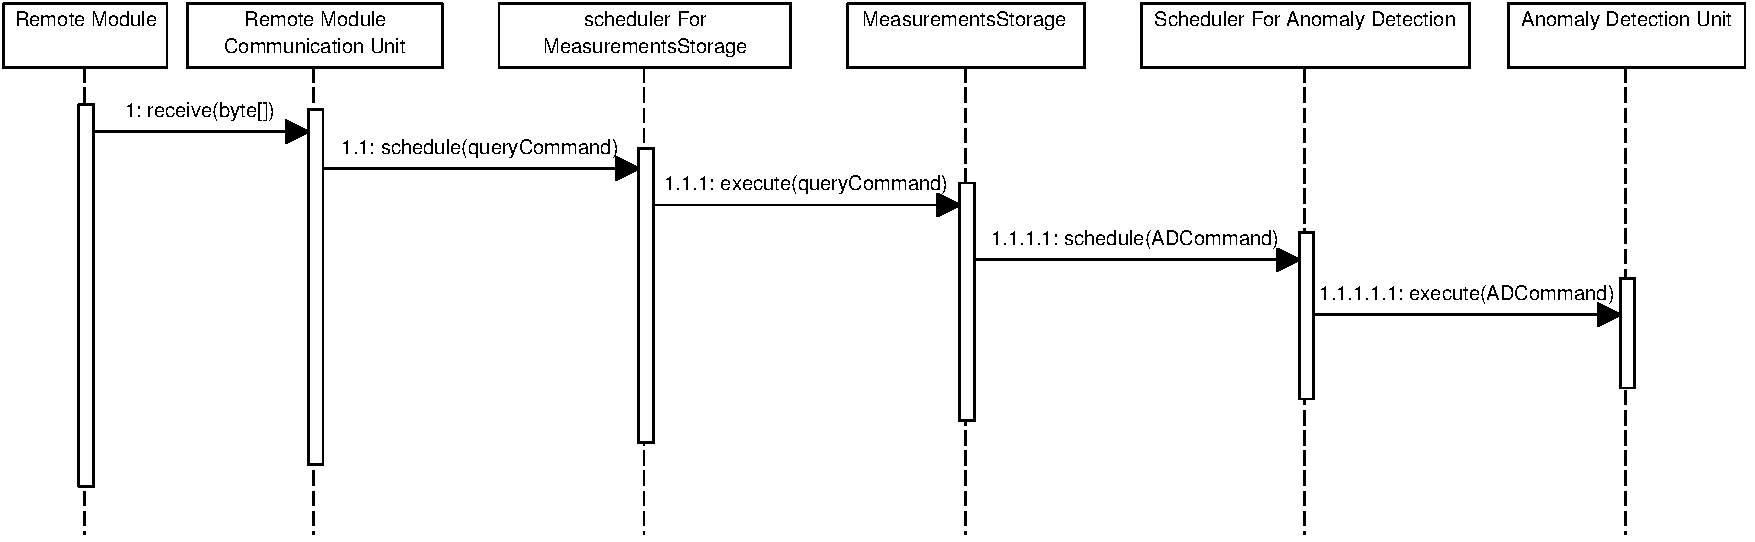
\includegraphics[width=\textwidth]{figs/scenario-5-6.pdf}
		\caption{The overview sequence diagram of scenario: Individual data analysis.}
		\label{fig:scenario-5-6}
	\end{centering}
\end{figure}

\begin{figure}
	\begin{centering}
		% TODO Figure
		%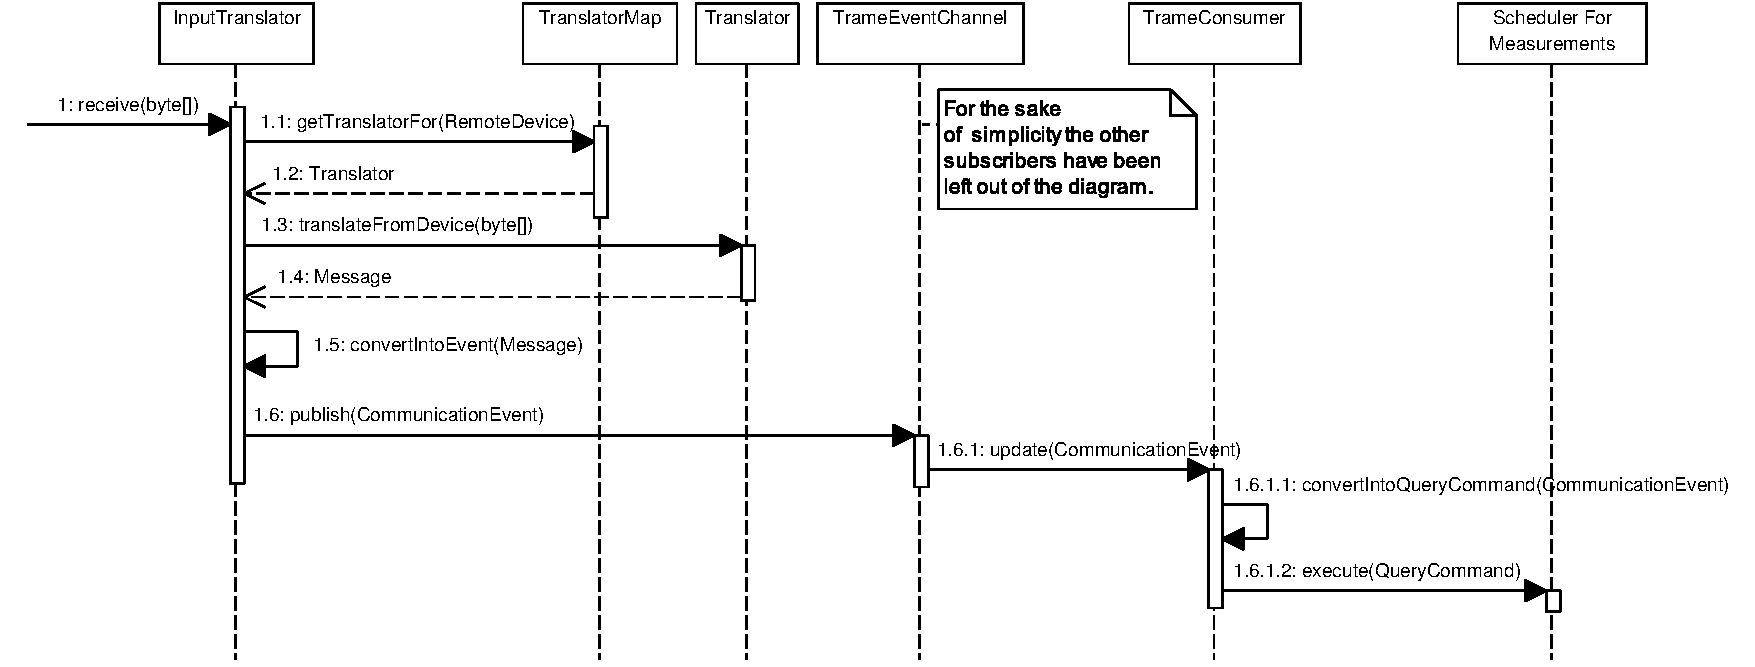
\includegraphics[width=\textwidth]{figs/scenario-5-6a.pdf}
		\caption{The sequence diagram zoomed in on the remote module communication
		unit.}
		\label{fig:scenario-5-6a}
	\end{centering}
\end{figure}

\begin{figure}
	\begin{centering}
		% TODO Figure
		%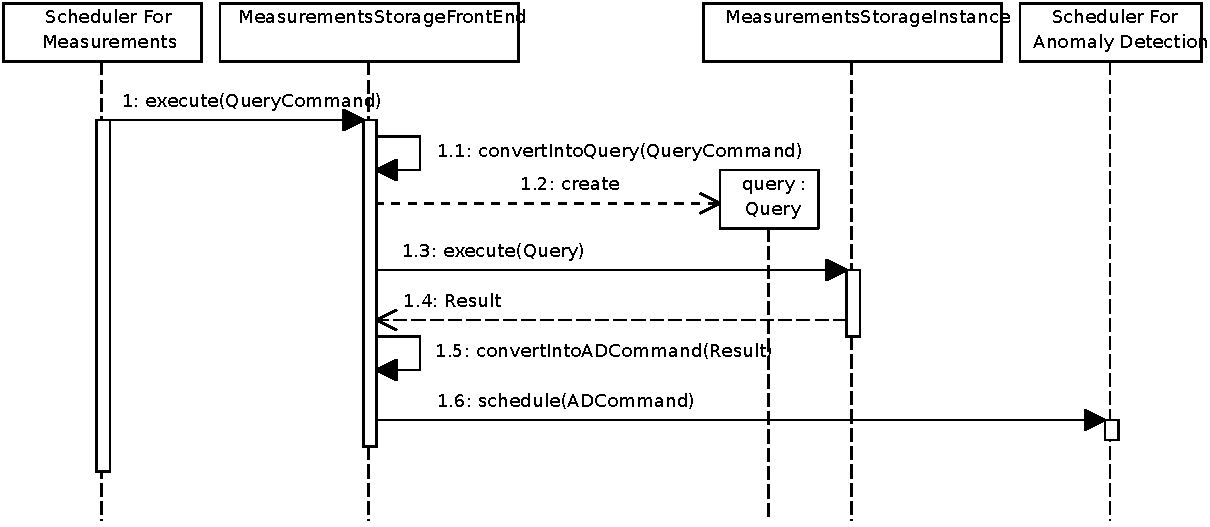
\includegraphics[width=\textwidth]{figs/scenario-5-6b.pdf}
		\caption{The sequence diagram zoomed in on the MeasurementsStorage.}
		\label{fig:scenario-5-6b}
	\end{centering}
\end{figure}

\npar The query in step 1.2 of figure \ref{fig:scenario-5-6b} is a store query
to store the incoming measurement.

\begin{figure}
	\begin{centering}
		% TODO Figure
		%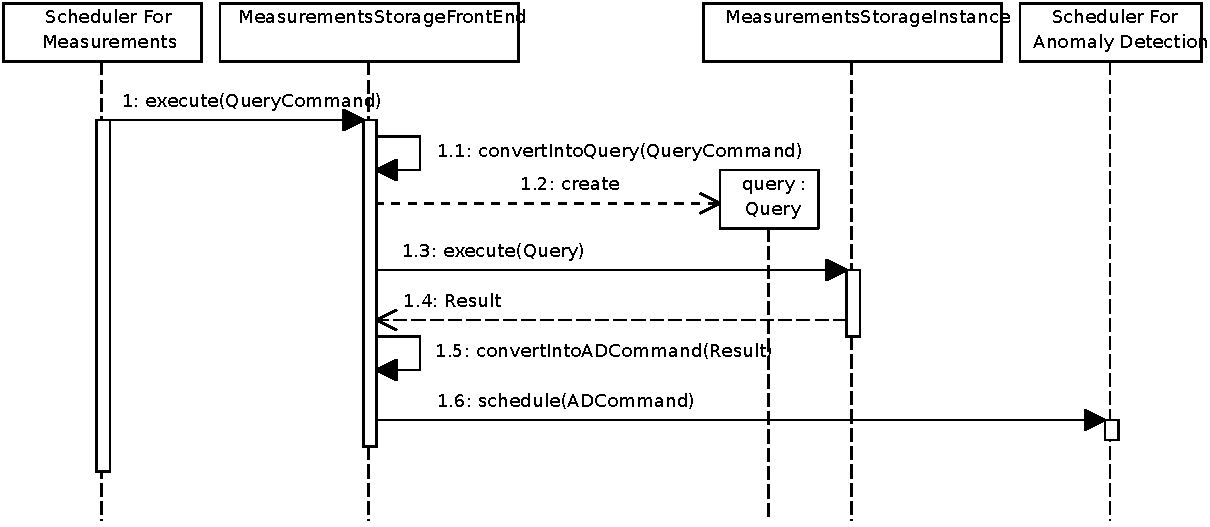
\includegraphics[width=\textwidth]{figs/scenario-5-6b.pdf}
		\caption{The sequence diagram zoomed in on the Anomaly Detection Unit.}
		\label{fig:scenario-5-6c}
	\end{centering}
\end{figure}

\npar In step 1.4 a read query is constructed to gain additional measurement
data belonging to the same remote module. The \method{addMeasurements()} method
will add the retrieved measurements to the ADCommand. In step 1.7 there is
another query constructed to store the results of the analysis. Once again this
means that the AlarmResult is empty.



